%%
%% This is file `sample-sigconf.tex',
%% generated with the docstrip utility.
%%
%% The original source files were:
%%
%% samples.dtx  (with options: `all,proceedings,bibtex,sigconf')
%%
%%
%% Commands for TeXCount
%TC:macro \cite [option:text,text]
%TC:macro \citep [option:text,text]
%TC:macro \citet [option:text,text]
%TC:envir table 0 1
%TC:envir table* 0 1
%TC:envir tabular [ignore] word
%TC:envir displaymath 0 word
%TC:envir math 0 word
%TC:envir comment 0 0
%%
\documentclass[sigconf]{acmart}

\AtBeginDocument{%
  \providecommand\BibTeX{{%
    Bib\TeX}}}

%% Rights management information — replace with values from ACM rights form
\setcopyright{acmlicensed}
\copyrightyear{2025}
\acmYear{2025}
\acmDOI{XXXXXXX.XXXXXXX}
\acmConference[SIGMOD '25]{ACM International Conference on Management of Data}{June 2025}{Berlin, Germany}
\acmISBN{978-1-4503-XXXX-X/2025/06}

%%\acmSubmissionID{123-A56-BU3}

\usepackage[utf8]{inputenc}
\usepackage[T1]{fontenc}
\usepackage{amsfonts}
\usepackage{amsmath}
\usepackage{booktabs}
\usepackage{microtype}
\usepackage{xcolor}
\usepackage{algorithm}
\usepackage{algpseudocode}
\usepackage{enumitem}

\begin{document}

\title{Influence Maximization under Sequential Coupon Diffusion}

%%
%% Authors and affiliations — replace with actual author information
%%
\author{Author One}
\authornote{Both authors contributed equally to this research.}
\email{author1@institution.edu}
\affiliation{%
  \institution{Institution Name}
  \city{City}
  \country{Country}
}

\author{Author Two}
\authornotemark[1]
\email{author2@institution.edu}
\affiliation{%
  \institution{Institution Name}
  \city{City}
  \country{Country}
}

\renewcommand{\shortauthors}{Author One et al.}

\begin{abstract}
Word-of-mouth and viral marketing have been extensively studied under classical influence propagation models such as Independent Cascade (IC) and Linear Threshold (LT), where activated nodes broadcast influence to all neighbors simultaneously. However, many real-world promotional campaigns --- such as digital coupon forwarding and invitation-code sharing --- follow a fundamentally different pattern: each piece of promotional content propagates as a single instance passed to at most one neighbor at each step. We formalize this setting as the \emph{Sequential Independent Diffusion Influence Maximization (SIDIM)} problem, where $k$ coupons are seeded and each propagates independently as a random walk. At each visited node, the coupon is either redeemed (activating the user and terminating the walk), discarded, or forwarded to exactly one neighbor. The objective is to select $k$ seed nodes that maximize the expected number of distinct users who redeem at least one coupon. We prove that SIDIM is NP-hard, and establish that the adoption spread function is monotone and submodular, admitting a greedy $(1-1/e)$-approximation. We further develop a tailored Reverse Influence Sampling (RIS) framework that jointly generates $k$ reverse reachable sets per root node, yielding a near-linear time algorithm with a $(1-1/e-\epsilon)$-approximation guarantee. Extensive experiments on real-world social networks validate both the importance of the SID formulation and the effectiveness of our approach.
\end{abstract}

%%
%% CCS concepts — generate at https://dl.acm.org/ccs/ccs.cfm
%%
\begin{CCSXML}
<ccs2012>
 <concept>
  <concept_id>10002951.10002952.10002953.10010820</concept_id>
  <concept_desc>Information systems~Social networks</concept_desc>
  <concept_significance>500</concept_significance>
 </concept>
 <concept>
  <concept_id>10003752.10003809.10010170.10010171</concept_id>
  <concept_desc>Theory of computation~Approximation algorithms analysis</concept_desc>
  <concept_significance>300</concept_significance>
 </concept>
</ccs2012>
\end{CCSXML}

\ccsdesc[500]{Information systems~Social networks}
\ccsdesc[300]{Theory of computation~Approximation algorithms analysis}

\keywords{influence maximization, viral marketing, coupon diffusion, random walk, reverse influence sampling, submodular optimization}

\maketitle

\section{Introduction}
\label{sec:intro}
Word-of-mouth and viral marketing techniques have become dominant strategies for product promotion in social networks. By selecting a small set of influential seed users, companies can trigger cascades of adoption along social connections, a problem commonly referred to as influence maximization (IM). Over the past two decades, IM has been extensively studied under classical models such as the Independent Cascade (IC) and Linear Threshold (LT) models, where activated nodes attempt to influence their neighbors in a broadcast manner. However, many real-world campaigns deviate from this paradigm. For example, when a retailer distributes digital coupons, a user who chooses not to redeem or discard the coupon may forward it to at most one other user. A similar pattern arises in invitation-code campaigns, where an inactive user can pass the code to only one specific friend. In both scenarios, the promotional content propagates via a sequential, one-to-one diffusion process. We refer to this setting as sequential influence diffusion (SID), which admits a formulation closely related to random walks on the social graph. Despite its practical relevance, this setting remains underexplored, with existing IM frameworks inherently tailored to broadcast diffusion and unable to capture such sequential propagation mechanisms.

This sequential propagation fundamentally alters both the diffusion mechanism and the objective landscape. First, the diffusion model is structurally different. In standard IC and LT models, an activated node attempts to influence all its neighbors simultaneously, resulting in a branching cascade that fans out rapidly across the network. In SID, however, each piece of promotional content is passed to at most one neighbor, tracing a chain-like propagation process through the network. Second, the definition of activation is strictly decoupled from mere exposure. In classical IM, a node is considered activated as soon as the message reaches it. In coupon or invitation-code scenarios, however, a node that simply forwards the coupon without using it is not considered activated; only a node that ultimately redeems the coupon counts as an activated user. Consequently, the intermediate nodes along the forwarding chain contribute nothing to the final activation. Third, since multiple coupons propagate independently, the same user may redeem more than one coupon, yet is counted as activated only once. The primary goal is therefore to maximize the number of distinct users who ultimately redeem at least one coupon, as each newly activated user represents a potential recurring customer. Beyond this, when multiple seeding strategies yield the same activation coverage, the total number of coupons redeemed also serves as an additional metric. These differences collectively fall outside the modeling scope of existing IM frameworks and call for a new problem formulation.

To address these challenges, we formalize the \emph{Sequential Independent Diffusion Influence Maximization (SIDIM)} problem. In our model, $k$ coupons are distributed to $k$ seed nodes, and each coupon propagates independently through the network as a random walk. At each node along the walk, one of three outcomes occurs: the node redeems the coupon and becomes activated, the node discards the coupon, or the node forwards the coupon to exactly one randomly selected neighbor. In the first two cases, the random walk terminates; in the third, it continues. The objective is to select $k$ seed nodes that maximize the expected number of distinct users who redeem at least one coupon. Since the $k$ coupons propagate independently, each coupon induces its own possible world along the nodes it may visit. The overall diffusion outcome is then determined by the joint configuration of $k$ independent possible worlds. We first prove that SIDIM is NP-hard, confirming the inherent computational intractability of the problem. We then analyze the structural properties of the objective function through the possible-world framework and establish that the expected adoption spread is monotone and submodular. This key property enables the application of a greedy algorithm with a $(1-1/e)$-approximation guarantee. To make the greedy algorithm scalable, we develop a novel Reverse Influence Sampling (RIS) framework tailored to the SID setting. Unlike classical RR set construction, where a single RR set captures all potential influence paths to a target node, our framework samples a number of reverse reachable sets proportional to the size of the node set --- one per coupon, corresponding to one per possible world --- reflecting the independent random walks in the diffusion process. Building on this RIS framework, we design a near-linear time seed selection algorithm with a $(1-1/e-\epsilon)$-approximation guarantee.

Our contributions are summarized as follows. First, we initiate the formal study of the SIDIM problem, a practically motivated yet theoretically underexplored setting that captures the single-path, multi-coupon nature of real-world sequential promotional campaigns. Second, we prove that SIDIM is NP-hard and establish that the adoption spread function is monotone and submodular, admitting a greedy algorithm with a $(1-1/e)$-approximation guarantee. Third, we develop a tailored RIS scheme that jointly generates $k$ reverse reachable sets per root node with provable unbiasedness, and build upon it a near-linear time algorithm with a $(1-1/e-\epsilon)$-approximation guarantee. Fourth, extensive experiments on real-world social networks demonstrate that our method significantly outperforms baselines adapted from classical IM, validating both the importance of the SID formulation and the effectiveness of our algorithmic framework.


\section{Related Work}

\paragraph{Influence maximization.}
The IM problem was first formulated by Domingos and Richardson~\cite{domingos2001mining,richardson2002mining}, who modeled viral marketing as probabilistic inference over a Markov random field. Kempe, Kleinberg, and Tardos~\cite{kempe2003maximizing} gave the foundational treatment: they introduced the IC and LT diffusion models, proved IM is NP-hard under both, and showed that the adoption spread function is monotone and submodular, enabling a greedy algorithm with a $(1-1/e)$-approximation guarantee. However, the greedy algorithm requires expensive Monte Carlo estimation of marginal gains. Leskovec et al.~\cite{leskovec2007celf} proposed the CELF optimization to exploit submodularity via lazy evaluations, reducing the number of function evaluations by orders of magnitude. Goyal, Lu, and Lakshmanan~\cite{goyal2011celf} further improved this with CELF++. Chen, Wang, and Yang~\cite{chen2009efficient} introduced the PMIA and LDAG heuristics to avoid Monte Carlo simulation entirely, at the cost of approximation quality.

\paragraph{Reverse influence sampling.}
Borgs et al.~\cite{borgs2014maximizing} made the decisive breakthrough by introducing the Reverse Influence Sampling (RIS) framework, which provides a $(1-1/e-\epsilon)$-approximation in expected near-linear time. Tang, Xiao, and Shi~\cite{tang2014influence} developed TIM and TIM+, the first practical RIS-based algorithms with rigorous sample complexity bounds. Tang, Shi, and Xiao~\cite{tang2015influence} subsequently introduced IMM, which tightens the sample complexity via a martingale stopping rule, achieving near-linear time with a significantly smaller constant. Nguyen, Thai, and Dinh~\cite{nguyen2016stop} proposed SSA and D-SSA, attaining asymptotically optimal sample complexity. Huang et al.~\cite{huang2017revisiting} revisited the analysis of these algorithms and identified conditions under which the sample bounds can be further tightened. Sun et al.~\cite{sun2018multi} extended the RIS paradigm to multi-round influence maximization, where $k$ seeds are deployed across successive rounds; although structurally distinct from our setting, their work similarly requires reasoning about $k$ independent propagation instances and informed our design of the $k$-joint RR set. All of these methods, however, are designed for the IC or LT broadcast model and assume that a single activated node can simultaneously influence all of its neighbors; they cannot be directly applied to the non-replicable SID setting we study.

\paragraph{Diffusion model variants.}
A substantial literature has extended the basic IC and LT models in various directions: competitive influence maximization~\cite{budak2011limiting}, location-aware diffusion~\cite{li2014efficient}, profit-maximizing seeding under cost constraints~\cite{lu2015competition}, and adaptive seeding where the seed set is expanded after observing early diffusion~\cite{seeman2013adaptive}. Despite their diversity, these models share the same broadcast diffusion paradigm: an activated node propagates influence to multiple neighbors simultaneously. Our model departs from this paradigm by having each coupon move as a single instance along a forwarding chain, terminating only when it is redeemed or discarded.

\paragraph{Random walks in networks.}
Random walks have been widely studied as a model for information spreading and node centrality~\cite{lovasz1993random}. PageRank~\cite{page1999pagerank} is the canonical example, computing a stationary distribution over a teleporting random walk. In the IM context, random walk centrality has been used as a heuristic seed selection criterion, but without formal approximation guarantees under a propagation model. Our work is the first to place random-walk-style propagation within the IM framework rigorously, exploiting the possible-world structure to define well-formed RR sets and establish the associated approximation guarantees.

\section{Problem Definition}

Let $G = (V, E)$ be a directed graph with $n = |V|$ nodes and $m = |E|$ edges, where a node $u \in V$ represents a user and a directed edge $(u, v) \in E$ indicates that $u$ may forward a coupon to $v$. Throughout this paper, we assume $G$ is strongly connected. Given a seed tuple $S = (s_1, s_2, \ldots, s_k) \in V^k$, a retailer distributes $k$ coupons, one to each seed user, and each coupon then propagates independently through the network according to the diffusion process described below.

Consider first the propagation of a single coupon. When a coupon arrives at a node $u$, one of three mutually exclusive outcomes occurs. With probability $p_u^a$, user $u$ \emph{adopts} the coupon: the coupon is redeemed, $u$ is marked as activated, and the propagation terminates at $u$. With probability $p_u^d$, user $u$ \emph{discards} the coupon: the coupon is removed from the network without activating anyone. With the remaining probability $p_u^t = 1 - p_u^a - p_u^d$, user $u$ \emph{transfers} the coupon to exactly one out-neighbor $v$, selected according to an edge-level forwarding parameter $p(u, v)$ satisfying $\sum_{v: (u, v) \in E} p(u, v) = p_u^t$. A crucial feature of this process, which sharply distinguishes our setting from classical IM models, is that the coupon itself is \emph{non-replicable}: unlike a piece of information in the IC or LT model that can be copied and broadcast to all neighbors simultaneously, a coupon exists as a single instance in the network and moves to at most one location at each step.

Building on this single-coupon process, the full diffusion proceeds by running $k$ such processes in parallel, one for each coupon-seed pair, with all stochastic decisions drawn independently across coupons. Because the $k$ coupons evolve independently, a node $u$ may be visited by multiple coupons during the overall diffusion, and may even adopt more than one of them. Yet from the retailer's standpoint, the same user being reached by several coupons is no more valuable than being reached by one. Accordingly, a user $u$ is considered ultimately \emph{activated} if at least one of the $k$ coupons is adopted at $u$, and is counted exactly once in the final outcome regardless of how many coupons reach or are redeemed by $u$.

\textit{Remark.} It is worth highlighting a subtle modeling distinction from classical IM. In the IC model, the activation along each edge is governed by an independent Bernoulli trial, and a node may be influenced through multiple edges in parallel. In our model, by contrast, the three outcomes a node faces upon receiving a coupon are \emph{mutually exclusive and competing for the same decision moment}: the user must choose between redeeming, discarding, or forwarding to a particular neighbor, and these choices share a common probability budget summing to one. This coupling between the three outcomes, together with the non-replicable nature of the coupon, is what gives rise to the chain-like propagation behavior characteristic of our setting.

\paragraph{Possible-world construction.}
To reason precisely about the diffusion outcome, we introduce an explicit possible-world construction. For each coupon $j \in [k]$ and each node $u \in V$, draw an independent sample $r_{u,j} \sim \mathrm{Uniform}[0,1]$. The outcome at $u$ in world $W_j$ is determined by:
\[
  \text{outcome}_{u,j} =
  \begin{cases}
    \text{adopt}   & \text{if } r_{u,j} \in [0,\; p_u^a], \\
    \text{discard} & \text{if } r_{u,j} \in (p_u^a,\; p_u^a + p_u^d], \\
    \text{transfer to } v & \text{if } r_{u,j} \in \bigl(p_u^a + p_u^d + \textstyle\sum_{w \prec v} p(u,w),\; p_u^a + p_u^d + \textstyle\sum_{w \preceq v} p(u,w)\bigr],
  \end{cases}
\]
where $w \prec v$ denotes the out-neighbors of $u$ preceding $v$ in a fixed ordering. The collection $W_j = \{r_{u,j}\}_{u \in V}$ constitutes the $j$-th possible world, and $\mathcal{W} = (W_1, \ldots, W_k)$ fully determines the diffusion outcome for all $k$ coupons.

\begin{definition}[Live edge]
An edge $(w, u) \in E$ is a \emph{live edge} in world $W_j$ if and only if $\mathrm{outcome}_{w,j} = \text{transfer to } u$, i.e., $r_{w,j}$ falls in the sub-interval of $[p_w^a + p_w^d, 1]$ that corresponds to forwarding specifically to $u$.
\end{definition}

Under this construction, node $u$ is activated by coupon $j$ seeded at $s_j$ if and only if:
\begin{enumerate}[label=(\roman*)]
  \item $r_{u,j} \leq p_u^a$, i.e., $u$ \emph{adopts} in world $W_j$ (event $A_{u,j}$); and
  \item there exists a directed path $s_j = w_0 \to w_1 \to \cdots \to w_l = u$ such that every edge $(w_i, w_{i+1})$ is a live edge in $W_j$.
\end{enumerate}
Condition~(ii) alone guarantees that every intermediate node $w_1, \ldots, w_{l-1}$ is in transfer state, since a live edge $(w, u)$ requires $\mathrm{outcome}_{w,j} = \text{transfer to }u$ by definition; no additional condition on intermediate nodes is necessary. We write $\mathrm{Adopt}_{u,j}(s_j)$ for the conjunction of (i) and (ii). Observe that $A_{u,j}$ is determined solely by $r_{u,j}$, whereas the live-edge path (ii) is determined by $\{r_{w,j}\}_{w \neq u}$; the two conditions are therefore \emph{stochastically independent} under the possible-world construction. The overall activation of $u$ is
\[
  \mathrm{Adopt}_u(S) \;=\; \bigvee_{j=1}^{k} \mathrm{Adopt}_{u,j}(s_j),
\]
and the \emph{adoption spread} $\sigma(S) = \sum_{u \in V} \Pr[\mathrm{Adopt}_u(S)]$ counts the expected number of distinct users who redeem at least one coupon. The optimization problem is formalized as:

\begin{definition}[SIDIM]
Given a directed graph $G = (V, E)$ with node parameters $\{(p_u^a, p_u^d)\}_{u \in V}$, edge forwarding parameters $\{p(u, v)\}_{(u, v) \in E}$, and an integer $k$, find an ordered seed tuple $S^*$ that maximizes the adoption spread:
\begin{equation}
S^* = \arg\max_{S \in V^k} \sigma(S).
\end{equation}
\end{definition}


\section{Complexity Analysis}

In this section, we analyze the computational complexity and structural properties of the SIDIM problem, which together motivate our algorithmic design in the next section.

\begin{theorem}
\label{thm:nphard}
The SIDIM problem is NP-hard.
\end{theorem}

\begin{proof}[Proof sketch]
The classical IM problem under the IC model can be cast as a special instance of our problem by setting $p_u^d = 0$ for every node $u$ and choosing the forwarding parameters $\{p(u, v)\}$ appropriately so that the resulting single-coupon walk reproduces an IC-style cascade restricted to a single trajectory. Since classical IM is NP-hard~\cite{kempe2003maximizing}, our problem is at least as hard. Full details are omitted for space.
\end{proof}

To analyze the structural properties of $\sigma(S)$, it is convenient to adopt a \emph{possible-world} perspective. For each coupon $j \in \{1, \ldots, k\}$ and each node $u \in V$, the stochastic outcome at $u$ when coupon $j$ visits it is encoded by a single uniform sample $r_{u,j}$, jointly determining $u$'s behavior (adopt, discard, or transfer) under coupon $j$. The collection of these samples across all nodes constitutes a possible world $W_j$, and the joint configuration $\mathcal{W} = (W_1, \ldots, W_k)$ of $k$ independent possible worlds fully determines the diffusion outcome. Within a fixed $\mathcal{W}$, whether $u$ is activated by seed tuple $S$ is a deterministic function of $S$, and $\sigma(S) = \mathbb{E}_{\mathcal{W}}\bigl[\sum_u \mathrm{Adopt}_u(S)\bigr]$.

\begin{theorem}
\label{thm:monosub}
The adoption spread $\sigma(S)$ is monotone non-decreasing and submodular in $S$.
\end{theorem}

\begin{proof}[Proof sketch]
Fix an arbitrary realization $\mathcal{W} = (W_1,\ldots,W_k)$. Under $\mathcal{W}$, define $T_u(\mathcal{W}) \subseteq V$ as the set of nodes $s$ such that placing coupon $j$ at $s$ would activate $u$ in world $W_j$ for some $j$ --- equivalently, the union of $j$-th reverse reachable sets of $u$ across worlds. Then $\mathrm{Adopt}_u(S)$ holds deterministically iff $S \cap T_u(\mathcal{W}) \neq \emptyset$.

Monotonicity is immediate: enlarging $S$ can only increase the chance that $S \cap T_u(\mathcal{W}) \neq \emptyset$. For submodularity, $S \mapsto \mathbb{I}[S \cap T_u(\mathcal{W}) \neq \emptyset]$ is a coverage function and hence submodular for any fixed $\mathcal{W}$. Summing over $u \in V$ and taking expectations over $\mathcal{W}$ preserves both properties, since they are closed under non-negative linear combinations. Therefore $\sigma(S)$ is monotone and submodular. Full details are omitted for space.
\end{proof}

Theorems~\ref{thm:nphard} and~\ref{thm:monosub} together characterize the SIDIM problem as a monotone submodular maximization problem subject to a cardinality constraint. By the classical result of Nemhauser et al.~\cite{nemhauser1978analysis}, a simple greedy algorithm that iteratively adds the node with the largest marginal gain achieves a $(1 - 1/e)$-approximation of the optimum. However, evaluating the marginal gain exactly is intractable, since computing $\sigma(S)$ for a given $S$ already requires reasoning over all possible worlds. In the next section, we develop a Reverse Influence Sampling framework tailored to the SID process, which estimates marginal gains efficiently and yields a near-linear time algorithm with a $(1 - 1/e - \epsilon)$-approximation guarantee.


\section{Algorithm}

\subsection{Greedy Baseline and Its Limitations}

The monotone submodularity of $\sigma(S)$ (Theorem~\ref{thm:monosub}) immediately yields a greedy algorithm: starting from $S = \emptyset$, iteratively add the node that maximizes the marginal gain $\Delta(v \mid S) = \sigma(S \cup \{v\}) - \sigma(S)$ until $|S| = k$. By~\cite{nemhauser1978analysis}, this achieves a $(1-1/e)$-approximation. However, computing $\sigma(S)$ exactly is \#P-hard, and even approximating it via Monte Carlo simulation requires $R$ independent $k$-coupon diffusion runs per candidate per greedy step. Let $\bar{L}$ denote the expected number of steps in one coupon walk; the total cost is $O(k^2 n R \bar{L})$, which is prohibitive for large networks. We therefore develop an efficient RIS-based algorithm.

\subsection{Reverse Reachable Sets for Coupon Diffusion}

We begin by adapting the reverse reachable (RR) set concept to the SID model.

\paragraph{Single-coupon reverse walk.}
Fix possible world $W_j$ for coupon $j$, in which each node $u$ has independently drawn a pre-determined action: adopt (with probability $p_u^a$), discard (with probability $p_u^d$), or forward to a specific out-neighbor $v$ (with probability $p(u,v)$ for each $(u,v)\in E$). The \emph{reverse reachable set} of target node $u$ under $W_j$ is defined as
\[
  R_j(u, W_j) =
  \begin{cases}
    \{w \in V \mid \exists\text{ a forwarding chain } w \to \cdots \to u \text{ in } W_j\} & \text{if } a_j(u) = \text{adopt}, \\
    \emptyset & \text{otherwise,}
  \end{cases}
\]
where a \emph{forwarding chain} $w_0 \to w_1 \to \cdots \to w_l = u$ in $W_j$ requires $a_j(w_i) = \text{forward-to-}w_{i+1}$ for all $i < l$, meaning no intermediate node absorbs the coupon before it reaches $u$.

\begin{lemma}
\label{lem:rr-coverage}
A seed $s$ activates node $u$ via coupon $j$ in possible world $W_j$ if and only if $s \in R_j(u, W_j)$.
\end{lemma}

\begin{proof}
Seed $s$ activates $u$ via coupon $j$ iff the forward walk from $s$ in $W_j$ reaches $u$ and $a_j(u) = \mathrm{adopt}$. Since the forward walk follows the deterministic forwarding chain in $W_j$, the walk from $s$ reaches $u$ iff there is a forwarding chain from $s$ to $u$ in $W_j$. Combined with the adoption condition, this is exactly the definition of $s \in R_j(u, W_j)$.
\end{proof}

\paragraph{The single-coupon case ($k=1$).}
When only one coupon is distributed to seed $s_1$, the adoption spread reduces to
\[
  \sigma(\{s_1\}) \;=\; \sum_{v \in V} \Pr\bigl[\mathrm{Adopt}_{v,1}(s_1)\bigr]
  \;=\; \sum_{v \in V} \Pr\bigl[s_1 \in R_1(v,W_1)\bigr]
  \;=\; n\cdot\mathbb{E}_{v\sim\mathrm{Uni}(V)}\bigl[\mathbb{I}[s_1 \in R_1(v,W_1)]\bigr],
\]
where the second equality applies Lemma~\ref{lem:rr-coverage}. This is exactly the classical RIS formula: uniformly sampling a root $v$ and checking whether $s_1$ belongs to $R_1(v,W_1)$ yields an unbiased estimate of $\sigma(\{s_1\})/n$. The independence of $A_{v,1}$ and the live-edge reachability yields an additional insight: rather than sampling $v$ uniformly, one may sample $v$ with probability proportional to $p_v^a$ and then generate the reachability structure of $R_1(v,W_1)$ without the adoption gate, reducing wasted samples in sparse-adoption networks.\footnote{This variance-reduction trick is especially valuable under high-forwarding conditions (Scenario~III, \S\ref{sec:exp-scenario}), where the average adoption probability $\bar{p}^a = n^{-1}\sum_v p_v^a$ can be as low as $0.01$--$0.06$. With uniform root sampling, the expected fraction of non-trivial (adoption-triggered) RR sets is $\bar{p}^a$, so the effective cost per useful sample is $1/\bar{p}^a$ times the generation cost --- a potential $16\times$--$100\times$ overhead. Importance-sampling $v \propto p_v^a$ eliminates this waste entirely while preserving unbiasedness; the corrected estimator is $\hat{\sigma}(\{s_1\}) = \bigl(\sum_v p_v^a\bigr) \cdot T^{-1}\sum_t \mathbb{I}[s_1 \in R_1(v^{(t)}, W_1^{(t)})]$ where no adoption gate is applied. We leave the extension of this optimization to the full $k$-coupon setting as future work.}

\paragraph{The general case: $k$ seeds and $k$ independent worlds.}
For $k$ coupons seeded at the ordered tuple $S = (s_1, \ldots, s_k)$, the $k$ worlds $W_1, \ldots, W_k$ are drawn independently. Node $v$ is activated if and only if at least one coupon activates it, i.e., $\mathrm{Adopt}_v(S) = \bigvee_{j=1}^k \{s_j \in R_j(v, W_j)\}$.
A critical subtlety distinguishes this from a naive union check: seed $s_j$ is \emph{coupled to world $W_j$} and can only activate $v$ through that world. Checking whether any seed in $S$ belongs to $\bigcup_j R_j(v, W_j)$ would allow seed $s_i$ ($i \neq j$) to ``use'' world $W_j$, overcounting the true activation probability. The correct indicator is
\[
  \mathbb{I}[\mathrm{Adopt}_v(S)] \;=\; \mathbb{I}\!\left[\bigvee_{j=1}^{k} \{s_j \in R_j(v,W_j)\}\right],
\]
where each $s_j$ is checked against its own world's RR set.

\begin{lemma}[Unbiasedness]
\label{lem:unbiased}
Let $v$ be drawn uniformly at random from $V$, and let $R_1(v), \ldots, R_k(v)$ be the corresponding reverse reachable sets sampled from $k$ independent worlds $W_1, \ldots, W_k$.  For any ordered seed tuple $S = (s_1, \ldots, s_k)$,
\[
  \mathbb{E}\!\left[\,\mathbb{I}\!\left[\bigvee_{j=1}^{k} \{s_j \in R_j(v)\}\right]\right]
  \;=\; \frac{\sigma(S)}{n}.
\]
\end{lemma}

\begin{proof}
\begin{align*}
  \mathbb{E}\!\left[\mathbb{I}\!\left[\bigvee_j \{s_j \in R_j(v)\}\right]\right]
  &= \frac{1}{n}\sum_{u \in V}
     \Pr\!\left[\bigvee_{j=1}^{k} \{s_j \in R_j(u,W_j)\}\right] \\
  &= \frac{1}{n}\sum_{u \in V}
     \Pr\!\left[\bigvee_{j=1}^{k} \mathrm{Adopt}_{u,j}(s_j)\right]
  \;=\; \frac{\sigma(S)}{n},
\end{align*}
where the second equality applies Lemma~\ref{lem:rr-coverage} and the independence of $W_1,\ldots,W_k$.
\end{proof}

\paragraph{Sampling procedure.}
Algorithm~\ref{alg:kernel} formalizes the single-node outcome as a deterministic function of the pre-sampled random number $r_{u,j}$.

\begin{algorithm}[t]
\caption{Single-Node Transition Kernel in World $W_j$}
\label{alg:kernel}
\begin{algorithmic}[1]
\Require Node $u$; coupon index $j$; $p_u^a$, $p_u^d$, $\{p(u,v)\}_{v:(u,v)\in E}$; random number $r_{u,j}$
\Ensure Outcome $(A_{u,j},\, D_{u,j},\, v^*)$ at node $u$
\If{$r_{u,j} \leq p_u^a$}
  \State \Return $(1,\; 0,\; \emptyset)$ \Comment{Adopt}
\ElsIf{$r_{u,j} \leq p_u^a + p_u^d$}
  \State \Return $(0,\; 1,\; \emptyset)$ \Comment{Discard}
\Else
  \State Let $v^*$ be the out-neighbor $v$ such that $r_{u,j}$ falls in $v$'s transfer interval
  \State \Return $(0,\; 0,\; v^*)$ \Comment{Transfer to $v^*$}
\EndIf
\end{algorithmic}
\end{algorithm}

Algorithm~\ref{alg:rrset} generates a single $k$-joint RR set for a uniformly drawn root $v$, using lazy random-number generation: $r_{w,j}$ is sampled on demand the first time node $w$ is encountered in world $j$, and reused thereafter. The algorithm first checks whether $v$ triggers an adopt event in any of the $k$ worlds; if no world produces an adopt, the sample contributes nothing to the coverage estimate and is discarded (zero-contribution rejection). For each world $j$ in which $v$ adopts, a backward BFS expands over live in-edges, collecting all nodes that can forward a coupon to $v$ along a live-edge path.

\begin{algorithm}[t]
\caption{Conditioned Union RR-Set Generation}
\label{alg:rrset}
\begin{algorithmic}[1]
\Require Graph $G=(V,E)$; $p_u^a$, $p_u^d$, $\{p(u,v)\}$ for all $u,v$; number of coupons $k$
\Ensure A union RR sample $Q(v, \mathcal{W})$, or $\emptyset$ if zero-contribution
\State Sample root $v$ uniformly from $V$
\State Sample $r_{v,1}, \ldots, r_{v,k} \sim \mathrm{Uniform}[0,1]$ independently
\For{$j = 1, \ldots, k$}
  \State $A_{v,j} \leftarrow \mathbb{I}[r_{v,j} \leq p_v^a]$
\EndFor
\If{$A_{v,j} = 0$ for all $j$}
  \State \Return $\emptyset$ \Comment{Zero-contribution: $v$ adopts in no world}
\EndIf
\State $Q \leftarrow \emptyset$
\For{$j = 1, \ldots, k$}
  \If{$A_{v,j} = 1$}
    \State $R_j \leftarrow \{v\}$;\ \ $\mathrm{queue} \leftarrow [v]$
    \While{$\mathrm{queue} \neq \emptyset$}
      \State $u \leftarrow \mathrm{queue.dequeue()}$
      \For{each in-neighbor $w$ of $u$ in $G$}
        \If{$r_{w,j}$ not yet sampled}
          \State Sample $r_{w,j} \sim \mathrm{Uniform}[0,1]$
        \EndIf
        \If{$(w, u)$ is a live edge in $W_j$ \textbf{ and } $w \notin R_j$}
          \State $R_j \leftarrow R_j \cup \{w\}$;\ \ $\mathrm{queue.enqueue}(w)$
        \EndIf
      \EndFor
    \EndWhile
    \State $Q \leftarrow Q \cup R_j$
  \EndIf
\EndFor
\State \Return $(Q,\; v)$
\end{algorithmic}
\end{algorithm}

\subsection{RIS-Optimized Algorithm}

Given $T$ independently sampled union RR sets $\{(Q^{(t)}, v^{(t)})\}_{t=1}^{T}$ produced by Algorithm~\ref{alg:rrset}, we select the $k$ seeds sequentially. In round $j$ ($j = 1, \ldots, k$), we use the $j$-th component RR sets $\{R_j^{(t)}\}_{t=1}^{T}$ to select seed $s_j$: choose the node $s_j$ that appears in the greatest number of these $j$-th-group RR sets, i.e.,
\[
  s_j = \arg\max_{u \in V}\; \bigl|\{t : u \in R_j^{(t)}\}\bigr|.
\]
This greedy selection maximizes the estimated marginal adoption spread contributed by coupon $j$ independently of the other coupons. Collecting $T$ union RR samples, the corrected adoption spread estimator is
\[
  \hat{\sigma}(S) = \frac{n}{T}\sum_{t=1}^{T}
    \mathbb{I}\!\left[\bigvee_{j=1}^{k} \bigl\{s_j \in R_j^{(t)}\bigr\}\right],
\]
which checks, for each sample $t$, whether \emph{the $j$-th seed $s_j$ belongs to the $j$-th component RR set $R_j^{(t)}$} — not whether any seed falls in the union $Q^{(t)}$. This per-coupon check is precisely what Lemma~\ref{lem:unbiased} proves to be unbiased: the union check $S \cap Q^{(t)} \neq \emptyset$ would over-count activations by allowing seed $s_j$ to ``borrow'' reachability from world $W_{j'}$ ($j' \neq j$), which is incorrect because world $W_j$ is the unique probability space in which coupon $j$ propagates. The required number of samples $T$ is determined by the IMM-style stopping criterion described below. The complete procedure is given in Algorithm~\ref{alg:risopt}.

We adapt the stopping criterion of IMM~\cite{tang2015influence}. Let
\[
  \lambda^* = \frac{(8 + 2\epsilon)\, n}{\epsilon^2}
  \left[(1-1/e)\sqrt{\ln\tbinom{n}{k} + \ln\tfrac{2}{\delta}} + \sqrt{\ln\tfrac{2}{\delta}}\right]^2.
\]
Algorithm~\ref{alg:risopt} doubles the RR set collection in phases and uses an empirical lower bound $\mathrm{LB}$ on the optimum to determine when $T = \lceil\lambda^*/\mathrm{LB}\rceil$ samples have been collected.

\begin{algorithm}[t]
\caption{RIS-Optimized$(G, k, \epsilon, \delta)$}
\label{alg:risopt}
\begin{algorithmic}[1]
\State $\mathcal{F} \leftarrow \emptyset$;\ \ $\mathrm{LB} \leftarrow 1$;\ \ $\epsilon' \leftarrow \epsilon/\sqrt{2}$
\For{$i = 1, \ldots, \lfloor\log_2 n\rfloor - 1$}
  \State $x \leftarrow n / 2^i$;\ \ $\theta_i \leftarrow \lambda^* / x$
  \While{$|\mathcal{F}| < \theta_i$}
    \State $\mathcal{F} \leftarrow \mathcal{F} \cup \{\text{Sample-}k\text{-Joint-RRSet}(G, k)\}$
  \EndWhile
  \State Greedy max-coverage on $\mathcal{F}$ $\Rightarrow$ seed tuple $S_i$
  \If{$\hat{\sigma}(S_i) \geq (1+\epsilon')\, x$}
    \State $\mathrm{LB} \leftarrow \hat{\sigma}(S_i)/(1+\epsilon')$;\ \ \textbf{break}
  \EndIf
\EndFor
\While{$|\mathcal{F}| < \lceil\lambda^*/\mathrm{LB}\rceil$}
  \State $\mathcal{F} \leftarrow \mathcal{F} \cup \{\text{Sample-}k\text{-Joint-RRSet}(G, k)\}$
\EndWhile
\State \Return greedy max-coverage on $\mathcal{F}$ with output $\hat{S}$
\end{algorithmic}
\end{algorithm}

\subsection{Theoretical Guarantees}

\begin{theorem}
\label{thm:approx}
With probability at least $1 - \delta$, Algorithm~\ref{alg:risopt} returns a seed tuple $\hat{S}$ satisfying
\[
  \sigma(\hat{S}) \;\geq\; (1 - 1/e - \epsilon)\cdot \sigma(S_{\mathrm{opt}}),
\]
and its expected running time is $O\!\left(\frac{k(k + \ell)(m + n)\log n}{\epsilon^2}\right)$, where $\ell = \log(1/\delta)$.
\end{theorem}

\begin{proof}[Proof sketch]
Let $\mathrm{OPT} = \sigma(S_{\mathrm{opt}})$ denote the optimal adoption spread.

\textit{Correctness.} Lemma~\ref{lem:unbiased} ensures unbiasedness of $\hat{\sigma}$. The greedy max-coverage step achieves a $(1-1/e)$ ratio on the sample objective. Using a random-variable version of the Chernoff bound (analogous to~\cite{tang2015influence}), one shows that with $T = \lceil\lambda^*/\mathrm{OPT}\rceil$ samples, $\hat{\sigma}(S_{\mathrm{opt}})$ concentrates within an $\epsilon'$ factor of $\mathrm{OPT}/n$ with probability $\geq 1-\delta/2$, and the greedy output $\hat{S}$ satisfies $\sigma(\hat{S}) \geq (1-1/e-\epsilon)\cdot \mathrm{OPT}$ with probability $\geq 1-\delta$.

\textit{Complexity.} The expected cost of one $k$-joint RR set is $O(k \cdot \mathbb{E}[|\text{single RR set}|])$. By an argument analogous to~\cite{borgs2014maximizing}, $\mathbb{E}[|\text{single RR set}|] = O((m+n)/n \cdot \mathrm{OPT}^{-1})$ under the coupon walk dynamics. With $T = O(\lambda^*/\mathrm{OPT})$ samples, the total expected work for RR set generation is $O(k \cdot (k+\ell)(m+n)\log n / \epsilon^2)$. Each greedy round over $\mathcal{F}$ costs $O(|\mathcal{F}|)$, contributing the same asymptotic term.
\end{proof}

\section{Experiments}

We evaluate RIS-Optimized on four real-world social networks under three diffusion scenarios, measuring both activation spread and total coupon redemptions. All experiments run on a machine with an Intel Xeon 2.4\,GHz processor and 128\,GB RAM; implementations are single-threaded.

\subsection{Experimental Setup}
\label{sec:exp-setup}

\paragraph{Datasets.}
Table~\ref{tab:datasets} lists five real-world networks. The four smaller graphs --- Netscience, NetFacebookEgo, DoubanRandom, and EmailEnron --- form our main evaluation suite, covering scientific collaboration, online social platforms, and email communication at scales from $379$ to $33{,}696$ nodes. The largest graph, \emph{network.douban} ($154{,}907$ nodes), is included in the table to illustrate the problem scale but is excluded from the oracle-based comparisons, since MC-CELF cannot complete on a graph of this size within a practical time budget. All graphs are treated as directed; undirected edges are split into two directed edges.

\begin{table}[t]
  \caption{Characteristics of the real-world datasets.}
  \label{tab:datasets}
  \centering
  \begin{tabular}{lrrrrr}
    \toprule
    Dataset         & $|V|$   & $|E|$     & Avg.\ deg. & Max out-deg. & Sparsity \\
    \midrule
    Netscience      & 379     & 1,828     & 4.82       & 34           & 98.72\% \\
    NetFacebookEgo  & 2,888   & 5,962     & 2.06       & 769          & 99.93\% \\
    DoubanRandom    & 4,723   & 11,774    & 2.49       & 45           & 99.95\% \\
    EmailEnron      & 33,696  & 361,622   & 10.73      & 1,383        & 99.97\% \\
    network.douban  & 154,907 & 654,206   & 4.22       & 287          & 99.97\% \\
    \bottomrule
  \end{tabular}
\end{table}

\paragraph{Diffusion parameters.}
Node probabilities are generated by the degree-based log-continuous procedure in Algorithm~\ref{alg:gendist}, which encodes the empirical tendency of high-degree nodes to forward more and adopt less. We evaluate three scenarios that stress-test distinct aspects of the coupon propagation process:

\begin{algorithm}[t]
\caption{Generate Degree-Based Node Probability Distributions}
\label{alg:gendist}
\begin{algorithmic}[1]
\Require Degree array $\{d_u\}_{u\in V}$; config $(\textit{base}_a, \textit{slope}_a, \textit{base}_d, \textit{slope}_d, h)$
\Ensure $\{p_u^a\}$, $\{p_u^d\}$, $\{p_u^t\}$ for all $u\in V$
\For{$u \in V$}
  \State $\hat{d}_u \leftarrow \min\!\bigl\{1,\max\{10^{-5}, \log(1+d_u)/\max_w\log(1+d_w)\}\bigr\}^h$
\EndFor
\For{$u \in V$}
  \State $p_u^a \leftarrow \textit{base}_a + \textit{slope}_a \cdot (1 - \hat{d}_u)$
  \Comment{Low-degree nodes adopt more}
  \State $p_u^d \leftarrow \textit{base}_d + \textit{slope}_d \cdot \hat{d}_u$
  \Comment{High-degree nodes discard more}
  \State $p_u^t \leftarrow 1 - p_u^a - p_u^d$
\EndFor
\State Set $p(u,v) = p_u^t / d_u$ uniformly across out-neighbors
\State \Return $\{(p_u^a, p_u^d, p_u^t)\}_{u\in V}$
\end{algorithmic}
\end{algorithm}

\begin{itemize}
  \item \textbf{Scenario~I (Normal)}: $\textit{base}_a=0.30$, $\textit{slope}_a=0.10$, $\textit{base}_d=0.10$, $\textit{slope}_d=0.10$, $h=1.0$. A balanced setting in which adoption and forwarding coexist at moderate rates, representative of a typical commercial coupon campaign.

  \item \textbf{Scenario~II (High Absorption)}: $\textit{base}_a=0.45$, $\textit{slope}_a=0.35$, $\textit{base}_d=0.15$, $\textit{slope}_d=0.05$, $h=1.0$. Expected absorption $\mathbb{E}[p_u^a + p_u^d] \approx 0.95$; mean transfer rate $\mathbb{E}[p_u^t] \leq 0.05$. Coupons terminate within one or two hops, so seed locality dominates.

  \item \textbf{Scenario~III (High Forwarding)}: $\textit{base}_a=0.01$, $\textit{slope}_a=0.05$, $\textit{base}_d=0.01$, $\textit{slope}_d=0.05$, $h=1.0$. Expected absorption $\mathbb{E}[p_u^a + p_u^d] \leq 0.12$; mean transfer rate $\mathbb{E}[p_u^t] \geq 0.88$. Coupons trace long random walks, amplifying the value of global coverage optimization.
\end{itemize}

\paragraph{Baselines.}
We compare RIS-Optimized against two groups of methods.

\smallskip\noindent\textit{Coupon-aware and structural heuristics.}
\begin{itemize}
  \item \textbf{MC-CELF}: Greedy seed selection with each marginal gain estimated by $10{,}000$ independent Monte Carlo simulations of the SID process, using CELF lazy evaluation~\cite{leskovec2007celf} to reduce function evaluations. This serves as the quality oracle.
  \item \textbf{1Hop-Sort}: Ranks each node $u$ by its expected one-step adoption score
    \[
      \mathrm{score}_{1h}(u) = p_u^a + \sum_{v \in N^+(u)} p(u,v)\, p_v^a,
    \]
    the probability that a coupon placed at $u$ is adopted within one forwarding step, then selects the top-$k$ nodes.
  \item \textbf{Alpha-Sort}: Ranks nodes by their own adoption probability $p_u^a$ in descending order and selects the top $k$.
  \item \textbf{DegreeTopM}: Selects the $k$ nodes with the highest out-degree, ignoring all probability parameters.
  \item \textbf{PageRank}~\cite{page1999pagerank}: Selects the $k$ nodes with the highest PageRank score.
  \item \textbf{Random}: Selects $k$ seeds uniformly at random; serves as the lower-bound reference.
\end{itemize}

\smallskip\noindent\textit{IC-model adaptations.}
\begin{itemize}
  \item \textbf{IMM}~\cite{tang2015influence}: The IMM algorithm applied to an IC-model interpretation of the graph, treating each edge weight $p(u,v)$ as an independent activation probability. Its inclusion tests whether a state-of-the-art IM solver can compensate for the fundamental model mismatch with SID propagation.
  \item \textbf{OPIM}~\cite{tang2018online}: An online-processing variant of IMM with improved practical efficiency, applied under the same IC interpretation.
\end{itemize}

\paragraph{Evaluation.}
Each seed set is evaluated by averaging the number of distinctly activated users over $10{,}000$ independent Monte Carlo simulations of the $k$-coupon diffusion process. We vary the seed budget $k$ from $1$ to $200$, reporting the full spread curve at all integer values.

\subsection{Adoption Spread under Normal Diffusion}
\label{sec:exp-normal}

Figure~\ref{fig:normal_spread} shows the expected number of activated users ($E[N_{\text{act}}]$) as a function of $k$ under Scenario~I across the four datasets. RIS-Optimized closely tracks the MC-CELF oracle at every value of $k$, validating the near-optimality of the RIS approximation for the SID model. Among the heuristics, 1Hop-Sort and Alpha-Sort perform substantially better than the topology-only methods (DegreeTopM, PageRank, Random), as they exploit the node-level adoption probabilities that govern the coupon walk. However, both coupon-aware heuristics fall increasingly short of RIS-Optimized as $k$ grows: without a global coverage objective, they seed redundant neighborhoods, whereas RIS-Optimized exploits the submodular structure to diversify seed placement across the network.

\begin{figure*}[t]
  \centering
  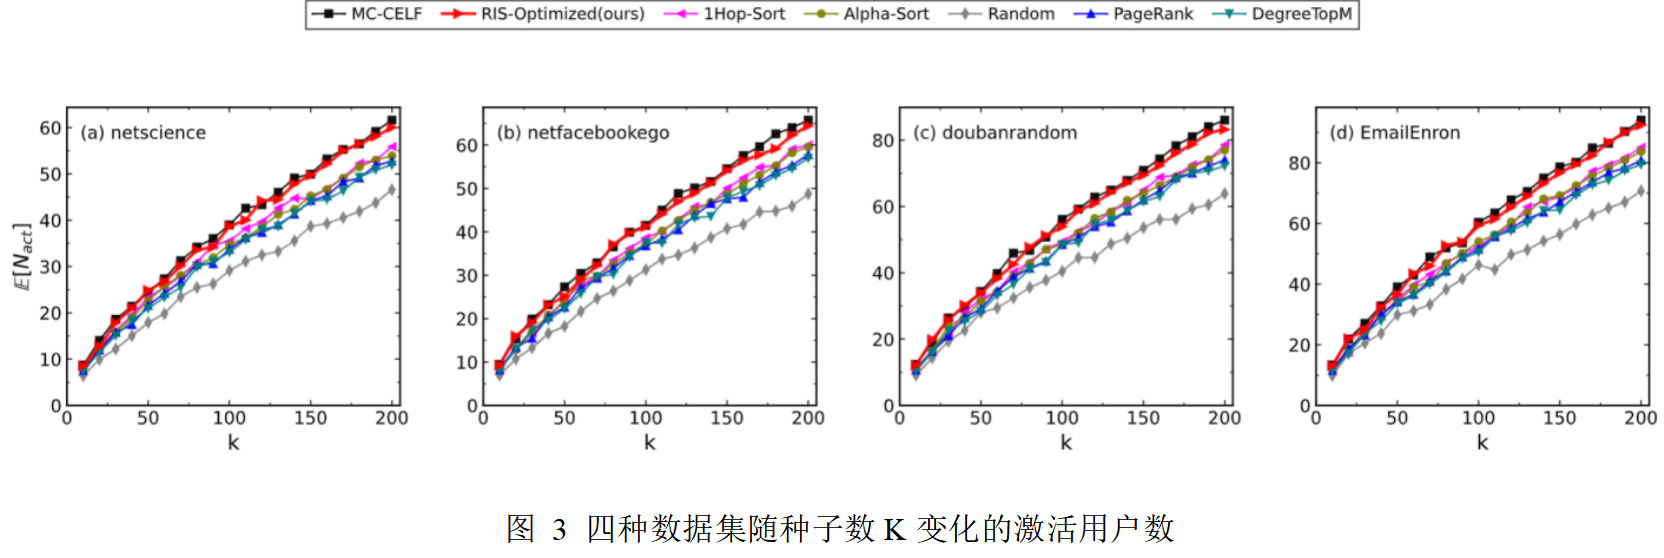
\includegraphics[width=\textwidth]{assets/fig_normal_spread}
  \caption{Expected number of activated users ($E[N_{\text{act}}]$) vs.\ seed budget $k$ under Scenario~I (Normal) across four datasets. RIS-Optimized closely tracks the MC-CELF oracle; coupon-aware heuristics (1Hop-Sort, Alpha-Sort) outperform topology-based baselines but fall behind RIS-Optimized as $k$ grows.}
  \label{fig:normal_spread}
\end{figure*}

Figure~\ref{fig:normal_redemp} reports the total number of coupons redeemed under the same conditions. As noted in the introduction, when two strategies yield similar activation coverage, the redemption count provides a secondary metric that captures how efficiently the coupon pool is consumed. The redemption curves closely mirror the activation-spread curves under Scenario~I --- indicating that most nodes adopt at most one coupon in the balanced setting --- yet RIS-Optimized leads on this secondary metric as well, confirming that the benefits of global spread optimization are not limited to unique-user coverage.

\begin{figure*}[t]
  \centering
  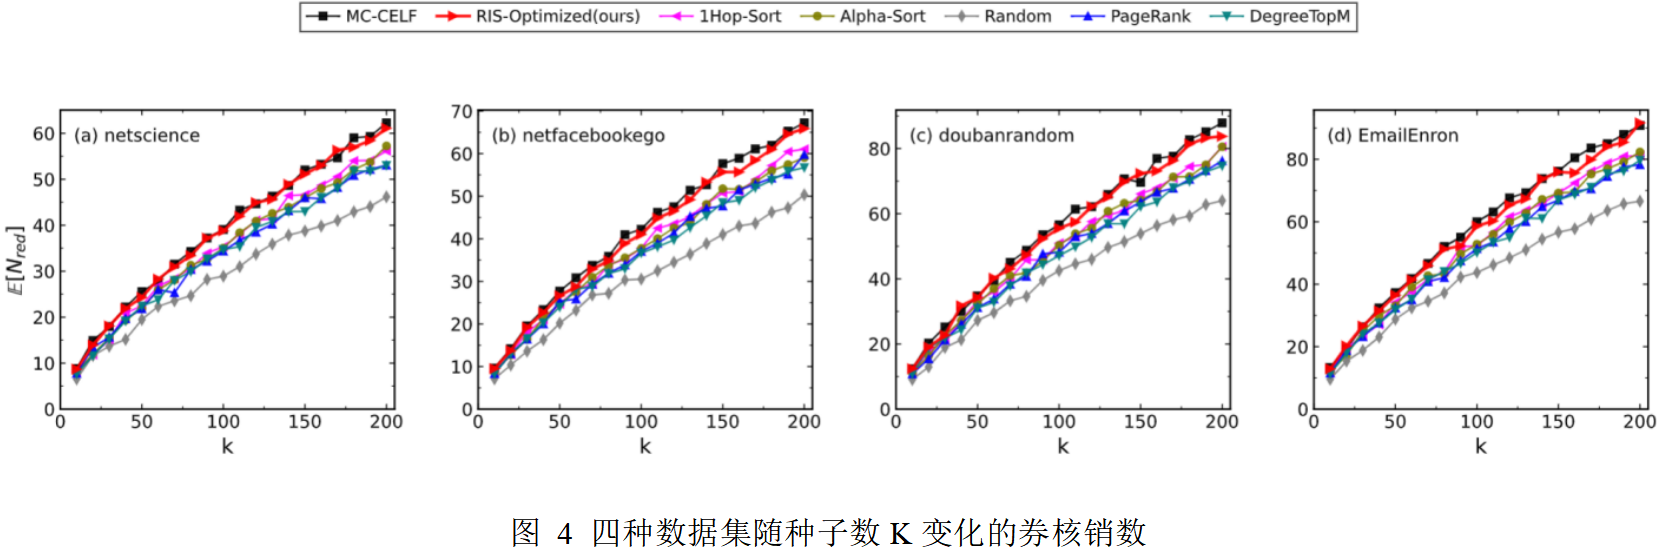
\includegraphics[width=\textwidth]{assets/fig_normal_redemption}
  \caption{Total coupon redemptions vs.\ $k$ under Scenario~I (Normal). The redemption curves closely mirror the activation-spread curves; RIS-Optimized leads under both primary and secondary metrics across all four datasets.}
  \label{fig:normal_redemp}
\end{figure*}

\subsection{Comparison with IC-Based Methods}
\label{sec:exp-ic}

Figure~\ref{fig:ic_compare} isolates the comparison between RIS-Optimized and the two IC-model baselines, IMM and OPIM. Across all four datasets and all values of $k$, RIS-Optimized achieves substantially higher activation spread. The underperformance of IMM and OPIM is not attributable to algorithmic weaknesses: both carry rigorous $(1-1/e-\epsilon)$-approximation guarantees for the IC model and their implementations are correct. The gap is instead a consequence of structural model mismatch. IC-based optimization selects seeds for their broadcast influence radius, favoring high-degree hubs that can simultaneously activate many neighbors; in SID propagation, however, a node can forward a coupon to only one neighbor, so degree confers no special propagation advantage. By contrast, RIS-Optimized is built around the actual single-path, random-walk dynamics of the coupon model and correctly identifies seeds that maximize adoption reach under this regime.

\begin{figure*}[t]
  \centering
  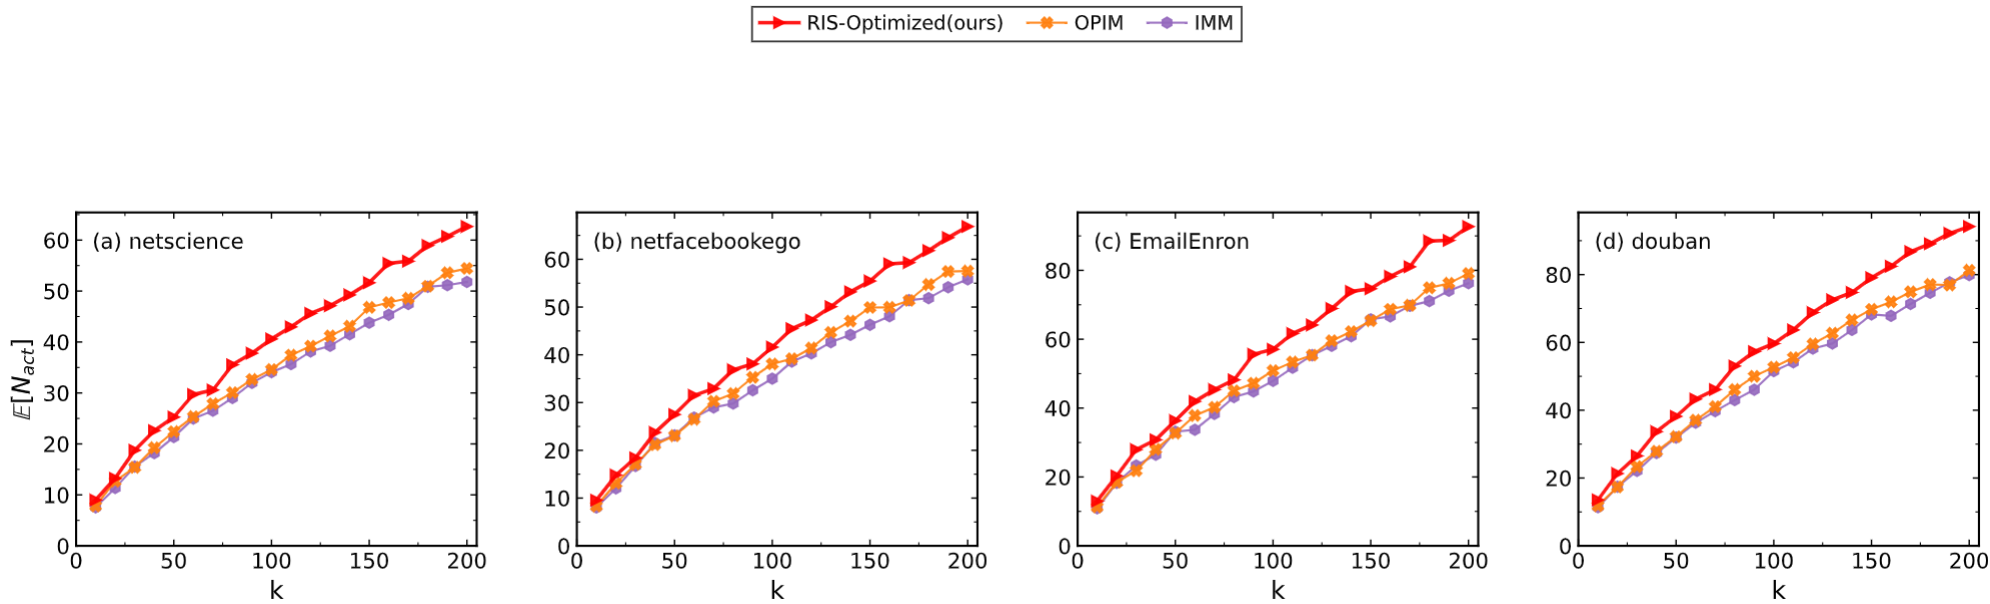
\includegraphics[width=\textwidth]{assets/fig_ic_comparison}
  \caption{Adoption spread of RIS-Optimized vs.\ IC-model baselines (IMM, OPIM) under Scenario~I (Normal). Despite their theoretical guarantees for the IC setting, IMM and OPIM consistently underperform because the broadcast-influence objective is structurally mismatched with SID propagation.}
  \label{fig:ic_compare}
\end{figure*}

\subsection{Effect of Diffusion Scenario}
\label{sec:exp-scenario}

Figures~\ref{fig:high_fwd} and~\ref{fig:high_abs} show activation spread under Scenario~III (High Forwarding) and Scenario~II (High Absorption), respectively.

\textbf{High Forwarding (Figure~\ref{fig:high_fwd}).}
With $\mathbb{E}[p_u^t] \geq 0.88$, coupons traverse long random-walk paths before being absorbed. Absolute spread values are lower than in Scenario~I because each node's per-visit adoption probability is very small, so coupons cover large graph distances without being redeemed. In this regime, global network topology becomes the decisive factor: seeds must be placed where random walks naturally converge toward high-adoption pockets of the network. RIS-Optimized maintains its lead over all baselines, and the gap relative to the coupon-aware heuristics 1Hop-Sort and Alpha-Sort is at least as pronounced as under Scenario~I, reflecting the insufficiency of one-hop adoption scores when walks are long.

\begin{figure*}[t]
  \centering
  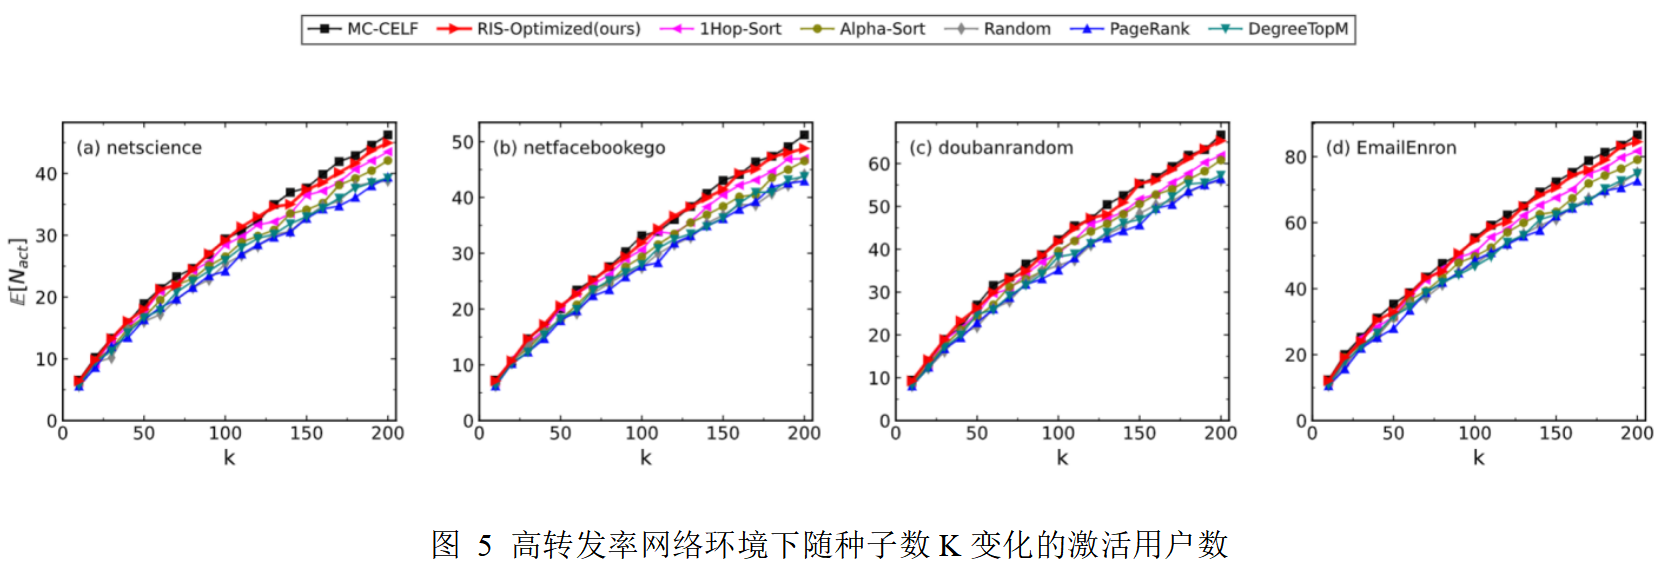
\includegraphics[width=\textwidth]{assets/fig_high_forwarding}
  \caption{Adoption spread vs.\ $k$ under Scenario~III (High Forwarding, $\mathbb{E}[p_u^t] \geq 0.88$). Long coupon walks amplify the importance of global coverage optimization; local heuristics fall further behind RIS-Optimized.}
  \label{fig:high_fwd}
\end{figure*}

\textbf{High Absorption (Figure~\ref{fig:high_abs}).}
With $\mathbb{E}[p_u^a + p_u^d] \approx 0.95$, coupons are absorbed within one or two hops of the seed. Absolute spread values are higher than in Scenario~I because the high per-visit adoption probability ensures that each seed's immediate neighborhood is reliably activated. Correspondingly, the spread curves from all methods are more tightly clustered: when propagation rarely extends beyond the first-hop neighbors, the optimization problem reduces nearly to covering as many distinct one-hop neighborhoods as possible, which even simple probability-based heuristics approximate well. RIS-Optimized continues to lead, but the margin over 1Hop-Sort and Alpha-Sort is narrower than in the other two scenarios, consistent with the reduced role of long-range structure.

\begin{figure*}[t]
  \centering
  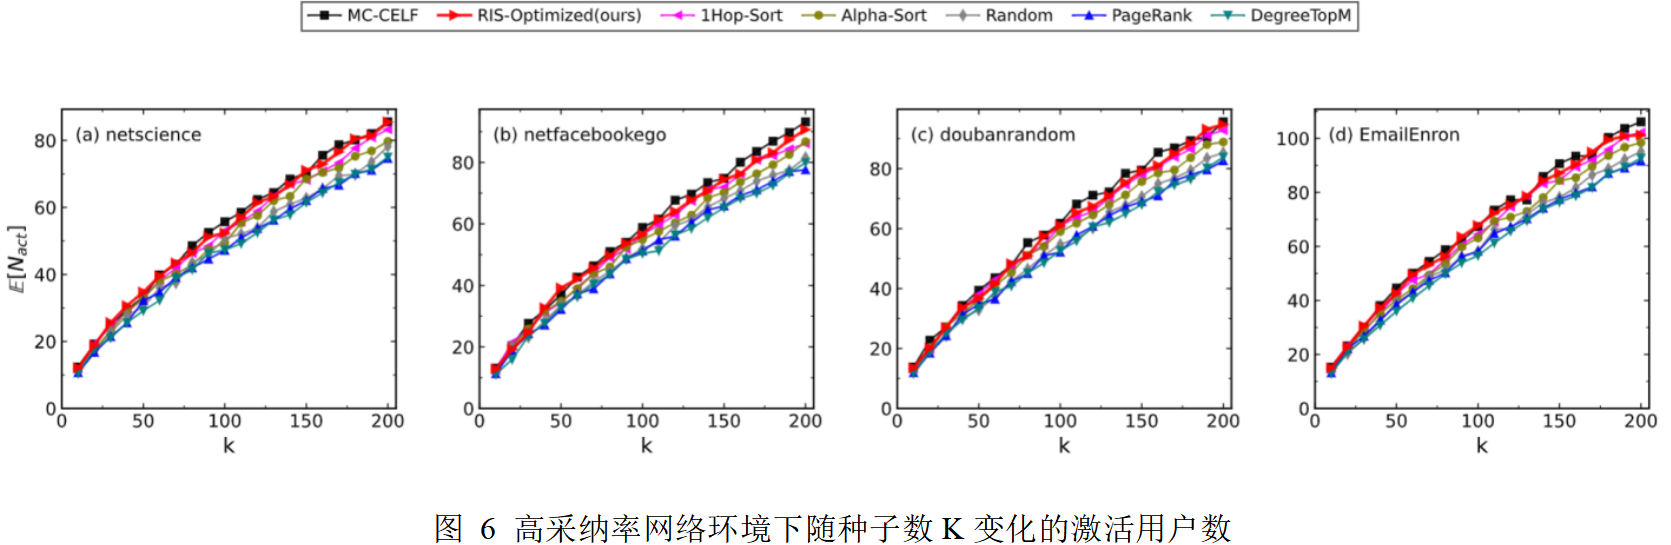
\includegraphics[width=\textwidth]{assets/fig_high_absorption}
  \caption{Adoption spread vs.\ $k$ under Scenario~II (High Absorption, $\mathbb{E}[p_u^a + p_u^d] \approx 0.95$). Short coupon walks reduce the importance of global coverage; methods are more tightly clustered, yet RIS-Optimized retains the lead.}
  \label{fig:high_abs}
\end{figure*}

\subsection{Running Time}
\label{sec:runtime}

Figure~\ref{fig:runtime} compares running time (milliseconds, log scale) as a function of $k$ across the four datasets. MC-CELF is omitted because its per-evaluation Monte Carlo cost makes it prohibitively slow even on the smallest graph; IMM and OPIM employ the same RIS sampling machinery as RIS-Optimized and incur comparable per-sample costs, so they are also omitted from this plot.

Alpha-Sort and 1Hop-Sort are the fastest methods, completing in roughly $10^2$\,ms regardless of $k$ or graph size: both reduce to a single linear scan over nodes followed by a sort, with no iterative computation. PageRank requires iterative power-method convergence, placing it in the $10^3$--$10^4$\,ms range on the larger graphs. RIS-Optimized incurs the highest cost among the plotted methods, reaching $10^4$--$10^5$\,ms on EmailEnron, reflecting the sampling budget needed to meet the $(1-1/e-\epsilon)$-approximation guarantee. Consistent with the $O(k(k+\ell)(m+n)\log n/\epsilon^2)$ bound of Theorem~\ref{thm:approx}, running time grows with both $k$ and graph size.

The results reveal a clear quality--efficiency trade-off. Alpha-Sort and 1Hop-Sort are fast but sacrifice spread quality, particularly at large $k$ and in the High Forwarding scenario. RIS-Optimized pays a higher computational price and in return matches the MC-CELF oracle. For the intended deployment setting --- offline seed selection ahead of a promotional campaign --- this cost is well justified.

\begin{figure*}[t]
  \centering
  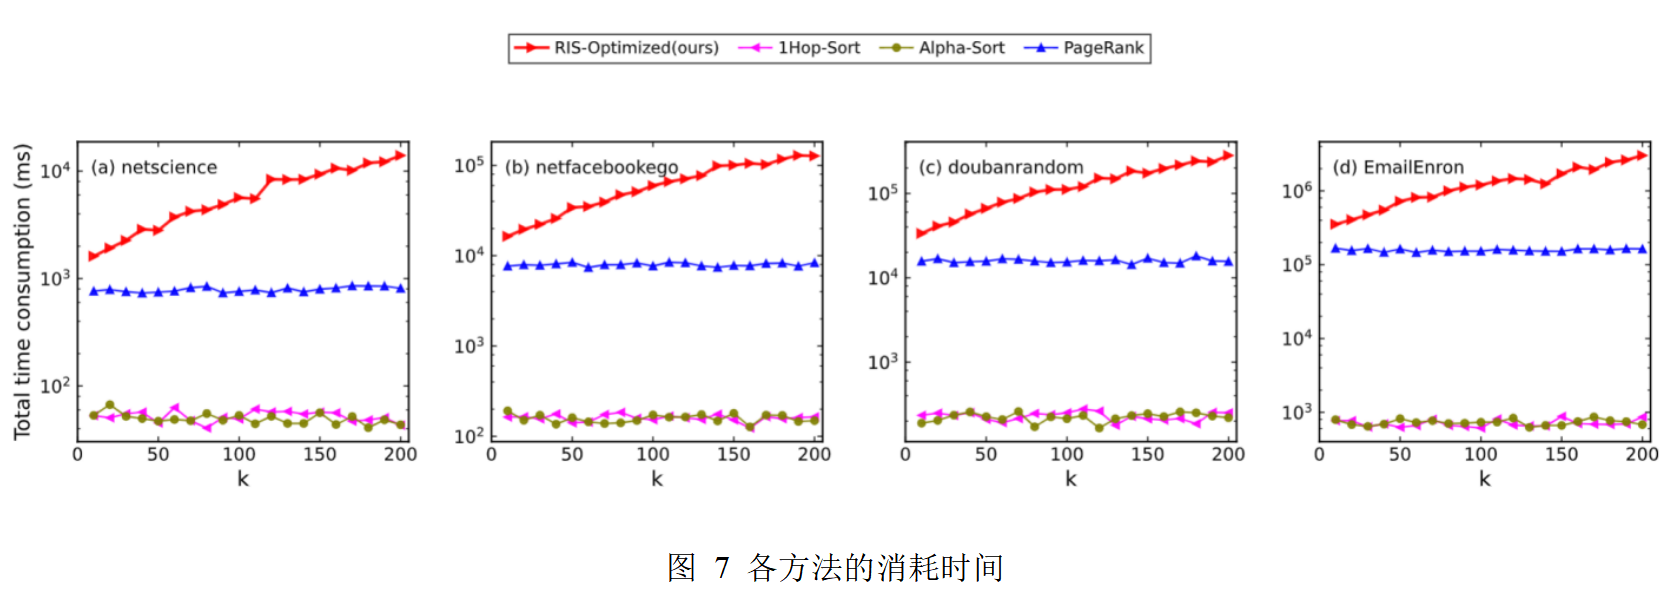
\includegraphics[width=\textwidth]{assets/fig_runtime}
  \caption{Total running time (ms, log scale) vs.\ seed budget $k$ across four datasets. Alpha-Sort and 1Hop-Sort complete in ${\sim}10^2$\,ms; PageRank in $10^3$--$10^4$\,ms; RIS-Optimized in $10^4$--$10^5$\,ms, reflecting the cost of the near-optimal approximation guarantee.}
  \label{fig:runtime}
\end{figure*}

\section{Conclusion}

We studied the Sequential Independent Diffusion Influence Maximization (SIDIM) problem, a practically motivated yet theoretically underexplored setting in which $k$ non-replicable coupons propagate through a social network as independent random walks. Unlike classical IM models where activated nodes broadcast influence to all neighbors, each coupon in our model traces a single forwarding chain and activates a user only upon redemption, not mere receipt. This distinction fundamentally changes both the diffusion mechanics and the optimization landscape.

We established that SIDIM is NP-hard and that the adoption spread function is monotone and submodular, admitting a greedy $(1-1/e)$-approximation. To make this tractable at scale, we developed a tailored Reverse Influence Sampling framework built on $k$-joint RR sets: for each target node, $k$ independent reverse random walks are sampled and they yield per-coupon unbiased estimators of each node's activation probability, enabling SIDIM to be cast as a maximum weighted coverage instance. This reduction to a maximum coverage instance allows RIS-Optimized to run in near-linear expected time while retaining a provable $(1-1/e-\epsilon)$-approximation guarantee. Experiments on four real-world networks confirm that RIS-Optimized closely matches the quality of the Monte Carlo oracle while outperforming classical IM adaptations and structural heuristics by a significant margin.

Several directions remain open. First, extending the model to heterogeneous forwarding behavior --- where different users apply different decision rules --- would better capture real campaign dynamics. Second, the current model assumes a static graph; incorporating temporal network evolution could yield more accurate predictions for time-sensitive promotional campaigns. Third, exploring budget-constrained variants, where seeds are allocated with non-uniform costs, is a natural next step toward practical deployment.

\begin{acks}
% Acknowledgments go here.
\end{acks}

\bibliographystyle{ACM-Reference-Format}
\bibliography{references}

\end{document}
